\documentclass[tikz]{standalone}
\usepackage{tikz} 
\usetikzlibrary{shapes.misc,patterns,hobby}
\usepackage{pgfplots}
\usepgfplotslibrary{fillbetween}
%\usepackage[active,tightpage]{preview}  %generates a tightly fitting border around the work
%\PreviewEnvironment{tikzpicture}
%\setlength\PreviewBorder{2mm}
\usepackage{xcolor}
\definecolor{myred}{RGB}{196,19,47} 
\definecolor{myblue}{RGB}{0,139,139}

\begin{document}
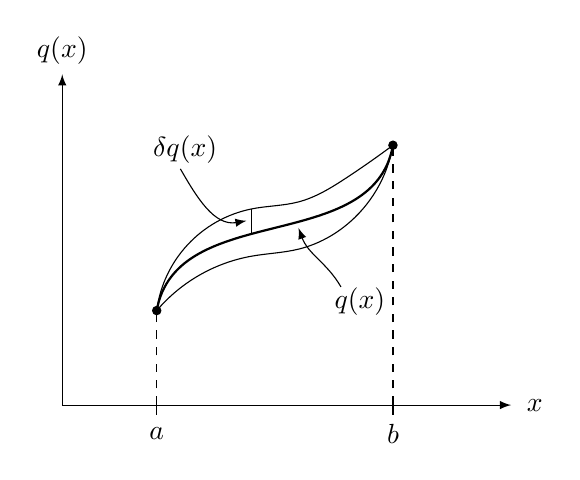
\begin{tikzpicture}[xscale=3,yscale=3,>=latex]

%Koordinatensystem (2D)
\draw[->, thin] (0,0) to (0,1.4);
\node at (0,1.5) {$q(x)$};
\draw[->, thin] (0,0) to (1.9,0);
\node at (2,0) {$x$};

\draw[-, thin] (0.4,-0.04) to (0.4,0.04);
\node at (0.4,-0.12) {$a$};
\draw[-, dashed] (0.4,0) to (0.4,0.4);
\draw[-, thin] (1.4,-0.04) to (1.4,0.04);
\node at (1.4,-0.12) {$b$};
\draw[-, dashed] (1.4,0) to (1.4,1.1);


\draw[-, thick] (0.4,0.4) [out=80, in=260] to (1.4,1.1);
\filldraw (0.4,0.4) circle (0.5pt); 
\draw[-] (0.4,0.4) to [curve through = { (0.8,0.83) (1,0.86) (1.2,0.96)  }] (1.4,1.1);
\draw[-] (0.4,0.4) to [curve through = { (0.8,0.63) (1,0.66) (1.2,0.76)  }] (1.4,1.1); 
\filldraw (1.4,1.1) circle (0.5pt); 


\draw[->, thin] (1.18,0.5) [out=120, in=290] to (1,0.75);
\node at (1.26,0.44) {$q(x)$};
\draw[-, thin] (0.8,0.72) to (0.8,0.83);
\draw[->, thin] (0.5,1) [out=300, in=190] to (0.78,0.78);
\node at (0.52,1.08) {$\delta q(x)$};


\end{tikzpicture}
\end{document}